%   __           _ _    _
%  / _|_   _ ___(_) | _| | __
% | |_| | | / __| | |/ / |/ /
% |  _| |_| \__ \ |   <|   <
% |_|  \__, |___/_|_|\_\_|\_\
%      |___/
\section{Physical theory of diffusion}\label{sec:physics}
Diffusion is simply the net movement of particles as a result of a random walk, and can be modelled as each atom constantly making a jump in a random  direction. It may seem a little counterintuitive that random motion can lead to a net flow, but consider that if there are \(10\) particles to the left, of which half move to the right, and \(100\) particles on the right, of which half move to the left, the net result is \(45\) particles moving to the left. The opposite of diffusion is drift, where the net motion is a result of an external driving force, for example an electric field.

The two most important equations in diffusion are Fick's laws, which, in one dimension, state that
\[
J = -D\pdv{C}{x} \qquad \qquad \pdv{C}{t} = D\pdv[2]{C}{x}
\]
where \(D\) is the diffusion coefficient, \(J\) the flux, i.e. the number of particles moving per area, and \(C\) the concentration, i.e. the number of particles per volume. Fick's second law, which is also simply called the diffusion equation, is the partial differential equation which is solved numerically on a dimensionless form in this project.


%  _____ _      _    _        __ _          _
% |  ___(_) ___| | _( )___   / _(_)_ __ ___| |_
% | |_  | |/ __| |/ /// __| | |_| | '__/ __| __|
% |  _| | | (__|   <  \__ \ |  _| | |  \__ \ |_
% |_|   |_|\___|_|\_\ |___/ |_| |_|_|  |___/\__|
\subsection{Derivation of Fick's first law in one dimension}
\begin{figure}[H]
    \centering
    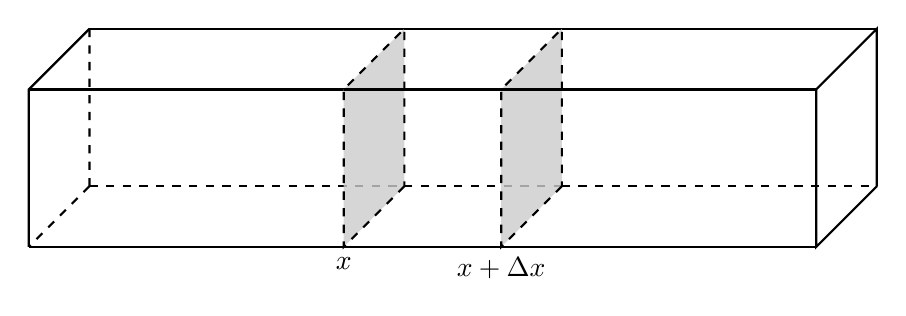
\begin{tikzpicture}[thick]
        \draw (0,0,2) -- (0,2,2) -- (0,2,0);
        \draw[dashed] (0,0,0) -- (0,0,2) (0,2,0) -- (0,0,0);
        \draw[dashed] (0,0,0) -- (4,0,0);
        \draw (0,0,2) -- (4,0,2);
        \draw (0,2,2) -- (4,2,2);
        \draw (0,2,0) -- (4,2,0);
        \fill[black!20!white,opacity=0.8] (4,0,0) -- (4,0,2) node[anchor=north] {\(x\)} -- (4,2,2) -- (4,2,0) -- (4,0,0);
        \draw[dashed] (4,0,0) -- (4,0,2) node[anchor=north] {\(x\)} -- (4,2,2) -- (4,2,0) -- (4,0,0);
        \draw[dashed] (6,0,0) -- (4,0,0);
        \draw (6,0,2) -- (4,0,2);
        \draw (6,2,2) -- (4,2,2);
        \draw (6,2,0) -- (4,2,0);
        \fill[black!20!white,opacity=0.8] (6,0,0) -- (6,0,2) -- (6,2,2) -- (6,2,0) -- (6,0,0);

        \draw[dashed] (6,0,0) -- (6,0,2) node[anchor=north] {\(x+\Delta x\)} -- (6,2,2) -- (6,2,0) -- (6,0,0);
        \draw[dashed] (6,0,0) -- (10,0,0);
        \draw (6,0,2) -- (10,0,2);
        \draw (6,2,2) -- (10,2,2);
        \draw (6,2,0) -- (10,2,0);
        \draw (10,0,0) -- (10,0,2) -- (10,2,2) -- (10,2,0) -- (10,0,0);
    \end{tikzpicture}
    \caption{Sketch of the infinitesimal volume element used in the derivation of Fick's laws in one dimension. Drawn in TikZ.}\label{fig:fick}
\end{figure}

As stated above, diffusion is the process of random walk. In one dimension, this means that each particle will have a \(\SI{50}{\percent}\) probability of moving one step to the left, and a \(\SI{50}{\percent}\) probability of moving one step to the right. As such, the net movement of particles to the right between \(x\) and \(x+\Delta x\) equals half the particles at point \(x\) minus half the particles at point \(x+\Delta x\). Since the flux is the movement of particles per cross-section area \(A\) (marked with grey in the figure) per time interval \(\Delta t\), this can be formulated mathematically as
\[
    J = -\frac{N(x+\Delta x, t) - N(x,t)}{2A\Delta t}
\]
Multiplying by \(\qty(\Delta x)^2\) in both the numerator and the denominator, and factoring out the \(\Delta t\), we get
\[
    J = -\frac{\qty(\Delta x)^2}{2\Delta t}\qty(\frac{N(x+\Delta x,t) - N(x,t)}{A\Delta x\cdot\Delta x})
\]
Since \(A\Delta x\) is a small volume element, \(C=N/\qty(A\Delta x)\):
\[
    J = -\frac{\qty(\Delta x)^2}{2\Delta t} \qty(\frac{C(x+\Delta x,t) - C(x,t)}{\Delta x})
\]
Defining \(D=\qty(\Delta x)^2/2\Delta t\) and letting \(\Delta x\to0\) gives Fick's first law:
\[
    J = -D\pdv{C}{x}
\]


%  _____ _      _    _                                    _
% |  ___(_) ___| | _( )___   ___  ___  ___ ___  _ __   __| |
% | |_  | |/ __| |/ /// __| / __|/ _ \/ __/ _ \| '_ \ / _` |
% |  _| | | (__|   <  \__ \ \__ \  __/ (_| (_) | | | | (_| |
% |_|   |_|\___|_|\_\ |___/ |___/\___|\___\___/|_| |_|\__,_|
\subsection{Derivation of Fick's second law in one dimension}
The derivation of Fick's second law is based on finding two different expressions for the change in the number of particles between \(x\) and \(x+\Delta x\), setting them equal to each other and inserting Fick's first law into the result.

To find the change in number of particles between the two grey surfaces in \vref{fig:fick} over a time interval \(\Delta t\), remember that the flux is defined as the number of particles passing per cross-section \(A\) per time interval \(\Delta t\). Therefore, the number of particles moving out of the volume between \(x\) and \(x+\Delta x\) in a time interval \(\Delta t\) is \(J(x+\Delta x,t)A\Delta t\), while the number of particles moving into the volume is \(J(x,t)A\Delta t\). Thus, the net change in the number of particles between \(x\) and \(\Delta x\) can be written as
\[
    \qty(J(x,t) - J(x + \Delta x,t))A\Delta t = -\qty(J(x+\Delta x,t) - J(x,t))A\Delta t
\]
On the other hand, this change in the number of particles must also equal the change in concentration, \(C(x,t+\Delta t) - C(x,t)\), multiplied with the volume, \(A\Delta x\). Since these two methods of calculating the change in the number of particles must give the same result, the following equation must hold:
\begin{alignat*}{2}
    -\qty(J(x+\Delta x,t) - J(x,t))A\Delta t &= \qty(C(x,t+\Delta t) - C(x,t)) A\Delta x\\
    \frac{J(x+\Delta x,t) - J(x,t)}{\Delta x} &= -\frac{C(x,t+\Delta t) - C(x,t)}{\Delta t}
\end{alignat*}
Letting \(\Delta x\to0\) and \(\Delta t\to0\), we get the so-called continuity equation:
\[
    \pdv{J}{x} = -\pdv{C}{t}
\]
Inserting Fick's first law for \(J\) on the left hand side, Fick's second law appears:
\begin{alignat*}{2}
    \pdv{x}\qty(-D\pdv{C}{x}) &= -\pdv{C}{t}\\
    D\pdv[2]{C}{x} &= \pdv{C}{t}
\end{alignat*}


%      _                 _             _        _
%  ___| |_ ___  __ _  __| |_   _   ___| |_ __ _| |_ ___
% / __| __/ _ \/ _` |/ _` | | | | / __| __/ _` | __/ _ \
% \__ \ ||  __/ (_| | (_| | |_| | \__ \ || (_| | ||  __/
% |___/\__\___|\__,_|\__,_|\__, | |___/\__\__,_|\__\___|
%                          |___/
\subsection{Steady state}\label{steadystate}
When \(t\to\infty\), the system will reach a steady state where the concentration at each point does not change with time. A different formulation is that for each volume element, the number of particles entering must be the same as the number of particles leaving, which means that the flux must be the same at all points. Using Fick's first law, this can be formulated as
\[
\text{constant} = J = -D\pdv{C}{x}
\]
which means that the concentration must be a linear function of \(x\). This is a test which both the analytical and the numerical solutions must pass.


%  _       _ _   _       _     _                           _
% (_)_ __ (_) |_(_) __ _| |   | |__   ___  _   _ _ __   __| | __ _ _ __ _   _
% | | '_ \| | __| |/ _` | |   | '_ \ / _ \| | | | '_ \ / _` |/ _` | '__| | | |
% | | | | | | |_| | (_| | |_  | |_) | (_) | |_| | | | | (_| | (_| | |  | |_| |
% |_|_| |_|_|\__|_|\__,_|_( ) |_.__/ \___/ \__,_|_| |_|\__,_|\__,_|_|   \__, |
%                         |/                                            |___/
\subsection{Initial and boundary conditions}
We will study a situation with a constant source at \(x=L\) and a drain at \(x=0\), with the system initially containing \(0\) particles everywhere but at the source. In the dimensionless form, this can be formulated as
\begin{alignat*}{6}
u(x,0) &= 0\qquad & x&\in\left[0,1\right)\\
u(0,t) &= 0\qquad & t&\in\mathbb{R}\\
u(L,t) &= 1\qquad & t&\in\mathbb{R}
\end{alignat*}
